\chapter{Resultados} \label{chap:resultados}
\textbf{Cinematica Directa}
\begin{figure} [h]
	\centering
	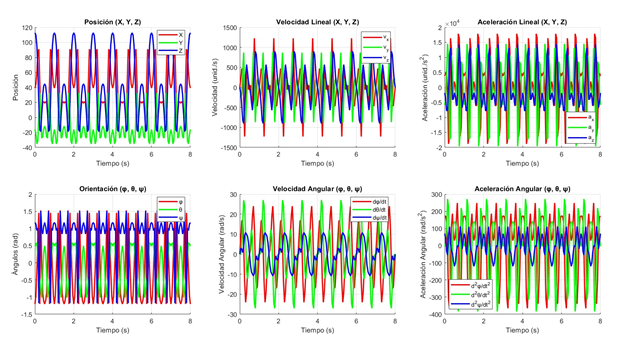
\includegraphics[width=0.7\linewidth]{img/cinematicadirecta}
	\caption{Cinematica directa}
	\label{fig:cinematicadirecta}
\end{figure}

\section*{Análisis de Resultados de Cinemática Directa}


\subsection*{1. Posición Lineal (X, Y, Z)}
La gráfica superior izquierda muestra el movimiento del efector final en los tres ejes cartesianos:


\begin{itemize}
	\item Se observa un movimiento cíclico y oscilatorio, lo que indica una trayectoria periódica en el espacio.
	\item El eje $Z$ (línea azul) tiene mayor amplitud, indicando un movimiento vertical más pronunciado.
\end{itemize}


\subsection*{2. Velocidad Lineal ($\dot{X}$, $\dot{Y}$, $\dot{Z}$)} La gráfica superior central presenta la velocidad en cada dirección:

\begin{itemize}
	\item Las señales son periódicas y muestran una alternancia entre valores positivos y negativos, coherente con el movimiento oscilatorio.
	\item La velocidad alcanza picos de aproximadamente ±1500 unidades/s, lo que indica variaciones rápidas en la trayectoria.
\end{itemize}


\subsection*{3. Aceleración Lineal ($\ddot{X}$, $\ddot{Y}$, $\ddot{Z}$)} La gráfica superior derecha representa la aceleración lineal:

\begin{itemize}
	\item Se observan valores muy altos (hasta ±2e4 unidades/s$^2$), lo que sugiere movimientos rápidos y posibles exigencias dinámicas considerables.
	\item Las aceleraciones son también periódicas y coinciden en fase con las velocidades.
\end{itemize}


\subsection*{4. Orientación (Ángulos de Euler $\phi$, $\theta$, $\psi$)} La gráfica inferior izquierda muestra la orientación del efector final:

\begin{itemize}
	\item Los ángulos de rotación (roll, pitch, yaw) también siguen trayectorias oscilantes.
	\item El ángulo $\phi$ (rojo) presenta las variaciones más marcadas.
\end{itemize}


\subsection*{5. Velocidad Angular}
La gráfica inferior central presenta las velocidades angulares derivadas de la orientación:


\begin{itemize}
	\item Se aprecian oscilaciones periódicas de baja frecuencia con amplitudes consistentes.
	\item Las señales presentan continuidad, lo cual es deseable para evitar movimientos abruptos.
\end{itemize}


\subsection*{6. Aceleración Angular}
Finalmente, la gráfica inferior derecha muestra las aceleraciones angulares:

\begin{itemize}
	\item Se mantiene el comportamiento periódico, pero con valores más elevados y picos que podrían afectar la estabilidad si no se amortiguan.
	\item Refleja las variaciones rápidas en la orientación del efector final.
\end{itemize}


\subsection*{Conclusión}
Este análisis permite verificar que el modelo de cinemática directa está proporcionando una trayectoria suave, periódica y coherente con el comportamiento esperado del robot. Las oscilaciones en posición, velocidad y aceleración indican que se está siguiendo un patrón cíclico, ideal para tareas repetitivas. No obstante, los picos de aceleración lineal y angular sugieren que se deben considerar estrategias de suavizado o limitación de esfuerzos en el diseño del control.

\textbf{Cinematica inversa}


\begin{figure} [h]
	\centering
	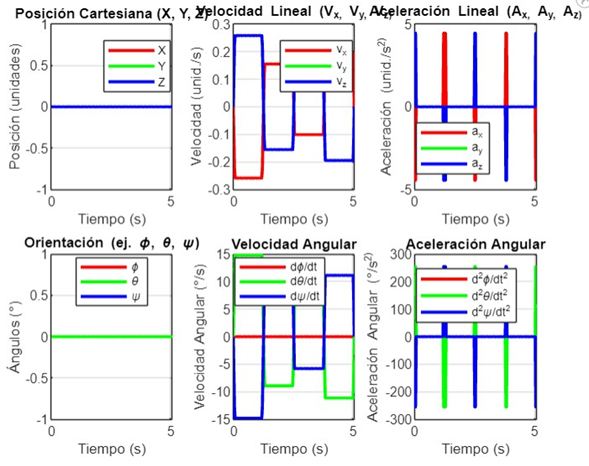
\includegraphics[width=0.7\linewidth]{img/cinematicainvgraficas}
	\caption{Cinematica inversa: Graficas}
	\label{fig:cinematicainvgraficas}
\end{figure}

\begin{figure} [h]
	\centering
	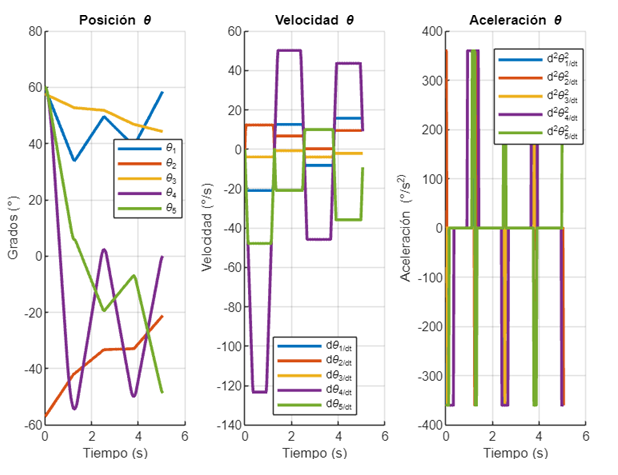
\includegraphics[width=0.7\linewidth]{img/cinematicainvarticular}
	\caption{Cinematica inversa: Articular}
	\label{fig:cinematicainvarticular}
\end{figure}

\newpage
\section*{Análisis de Resultados de Cinemática Inversa}


\subsection*{1. Posición angular $\theta$}
Esta gráfica muestra la posición angular (en grados) de cada articulación en función del tiempo. Cada curva representa el comportamiento de una articulación:


\begin{itemize}
	\item Se observa que las trayectorias son distintas para cada articulación, lo cual indica que cada una realiza un movimiento específico para contribuir al seguimiento de la trayectoria deseada del efector final.
	\item Por ejemplo, $\theta_4$ (línea morada) presenta cambios abruptos y amplios, sugiriendo que dicha articulación realiza movimientos significativos.
\end{itemize}


\subsection*{2. Velocidad angular $\frac{d\theta}{dt}$}

Esta gráfica representa la velocidad angular de las articulaciones (en grados por segundo):


\begin{itemize}
	\item Se observan escalones en las velocidades, indicando que fueron obtenidas mediante diferencias finitas sobre datos muestreados.
	\item Cambios bruscos de velocidad, especialmente en $\theta_4$ y $\theta_5$, pueden generar problemas de control o desgaste mecánico si no se suavizan.
\end{itemize}


\subsection*{3. Aceleración angular $\frac{d^2\theta}{dt^2}$}
La tercera gráfica muestra la aceleración angular (en grados por segundo cuadrado):


\begin{itemize}
	\item Se aprecian valores muy altos (por ejemplo, $\pm 360~^\circ/s^2$), lo que indica transiciones rápidas en la velocidad angular.
	\item Estas aceleraciones escalonadas también sugieren una obtención por diferencias finitas.
	\item Tales picos podrían ser perjudiciales para la operación del robot si no se implementa una trayectoria más suave.
\end{itemize}


\subsection*{Conclusión}
Las gráficas reflejan el comportamiento articular necesario para seguir una trayectoria en el espacio cartesiano. Sin embargo, los cambios abruptos en velocidad y aceleración
indican la necesidad de aplicar técnicas de suavizado como interpolación polinómica (por ejemplo, polinomios cúbicos o quínticos) para garantizar un movimiento más eficiente, seguro y adecuado para el control del robot.


\section*{Análisis de Resultados de Cinemática Inversa Articular}
	
	\section*{Gráfica 1: Posición angular ($\theta$)}
	
	\begin{itemize}
		\item \textbf{Eje X (Tiempo en segundos)}: Representa la evolución temporal (0 a 6 segundos).
		\item \textbf{Eje Y (Grados °)}: Muestra la posición angular de cada articulación en grados.
		\item \textbf{Curvas ($\theta_1$ a $\theta_5$)}: Indican cómo cambian los ángulos articulares en el tiempo.
	\end{itemize}
	
	\textbf{Interpretación:}
	\begin{itemize}
		\item Se observan trayectorias distintas para cada articulación, lo que implica que el movimiento fue calculado individualmente para lograr un posicionamiento específico del efector final (probablemente un robot).
		\item Algunas curvas son suaves, otras muestran cambios abruptos, lo cual puede indicar trayectorias con quiebres o cambios de dirección.
	\end{itemize}
	
	
	\section*{Gráfica 2: Velocidad angular ($d\theta/dt$)}
	
	\begin{itemize}
		\item \textbf{Eje X}: Tiempo (s)
		\item \textbf{Eje Y}: Velocidad angular (°/s)
		\item \textbf{Curvas}: Derivadas de las posiciones angulares (velocidades instantáneas).
	\end{itemize}
	
	\textbf{Interpretación:}
	\begin{itemize}
		\item Se observan velocidades constantes por tramos (formas tipo escalón), lo que indica movimiento a velocidad constante en ciertos intervalos, típico en trayectorias por segmentos lineales.
		\item Cambios abruptos implican transiciones entre movimientos.
	\end{itemize}
	
	
	\section*{Gráfica 3: Aceleración angular ($d^2\theta/dt^2$)}
	
	\begin{itemize}
		\item \textbf{Eje X}: Tiempo (s)
		\item \textbf{Eje Y}: Aceleración angular (°/s²)
		\item \textbf{Curvas}: Segunda derivada de la posición, muestran cómo cambia la velocidad en el tiempo.
	\end{itemize}
	
	\textbf{Interpretación:}
	\begin{itemize}
		\item Aceleraciones son valores muy altos positivos y negativos en intervalos muy breves, lo que sugiere cambios instantáneos de velocidad (lo cual no es físicamente ideal).
		\item Estos picos pueden indicar falta de suavizado en la planificación del movimiento.
	\end{itemize}
	
	
	\section*{Conclusión}
	
	Este conjunto de gráficas parece derivarse de una planificación de trayectorias por puntos (p. ej., control punto a punto en un robot articulado), donde se definieron posiciones deseadas de las articulaciones y se calcularon las velocidades y aceleraciones mediante diferencias finitas.
	
	\textbf{Posibles aplicaciones:}
	\begin{itemize}
		\item Control de robots manipuladores (como brazos robóticos).
		\item Simulación de trayectorias para verificación antes de ejecución física.
		\item Evaluación de la suavidad del movimiento.
	\end{itemize}
	

